\documentclass[../dissertation.tex]{subfiles}
\begin{document}

\chapter{Design}
\label{chap:design}

\section{Scope of the System}
\label{sec:scope}

\subsection{Overview}

The first necessary step was to decide how the server would interact with networks. Given that Tulip was considered the best software under the criteria tested for in Section \ref{sec:systematic-review}, a possibility would be to use the APIs that Tulip provides. Tulip provides both a C++ API \cite{tulipcppapi} and Python API \cite{tulippyapi} (of which the Python API is a wrapper around the C++ API), so the web application could be made using either of the languages. As ``Python is very flexible and makes experimentation easy'' \cite{zelle2004python}, and additionally Python has a popular web framework, Django \cite{django}, which is ``a powerful Web application framework that lets you do everything rapidly — from designing and developing the original application to updating its features'' \cite{forcier2008python}, this seemed a reasonable choice of stack to develop on. Additionally, this stack allows for the flexibility of Python and the power of C++, which makes it ideal for processing massive networks. It is worth noting that Tulip has covered web visualisations before, when its creators visualised the Firefox Dataset as part of a competition \cite{tulipfirefox}. However, this was an isolated project and currently there is no supported web visualisation framework made by Tulip.

The application that was hence to be created was to use:

\begin{itemize}
    \item A Django Web Framework
    \item A database that was to be created and maintained by Django
    \item A Tulip Python API Web Wrapper that would be called by Django and make calls to Tulip
    \item A front-end JavaScript library to interface with the Django web framework, allowing for the uploading, viewing and deletion of networks
    \item A JavaScript network visualisation framework
\end{itemize}

\subsection{Back-end}
\label{sec:overview-backend}

The back-end would consist of Django, the database it creates, the Tulip Python API (which is a wrapper around the Tulip C++ API) Web Wrapper, and the possible ability to connect to an external file host. This would enable it to be expandable to as many users as the host deemed necessary.

The main Django app (and database it creates) would include the logic for the server. This involves setting up the project \texttt{urls} file, which maps each url to a view, then each \texttt{view} has to be created which dictates what is returned to the client, whether a simple text response that is rendered, or a JsonResponse that returns data to an API call. Additionally, both models and forms would have to be created, which define what objects can be stored in the database, and how they are uploaded to the server.

The Tulip Python API Web Wrapper (itself a REST API) would include a number of functions that can be called from the front-end of the app, and would take in any necessary parameters and pass them to the Tulip Python API. A REST API is ``the face of a web service, directly listening and responding to client requests'' \cite{masse2011rest}. The main purpose of this would be so that when a network gets loaded, instead of sending it directly to the front-end to be rendered, it is optimised in some way first and then sent to the client in a reduced form which will both mean the network will be transferred faster to the client and then visualised faster too. It was decided that there would be three ways to optimise the information that was to be sent:
\begin{enumerate}
    \item \textbf{Node pruning.} This is removing each node with one edge from the network.
    \item \textbf{Node bundling based on cliques.} This is based on selecting nodes whose neighbours are highly interconnected and results on the selected node having those neighbours bundled into it.
    \item \textbf{Node bundling by number of edges.} This is based on finding nodes with the most edges and bundling each node connected to it into it.
\end{enumerate}

The web wrapper could be made exactly to match what functions the front-end requires, but a far more elegant and reusable solution would be to make it as flexible and as full as possible, allowing developers to have as much freedom as possible, and not have their options limited by the web wrapper's API. For this project it is likely that the flexibility of the web wrapper would be prioritised over the number of features, given time constraints, although at a later date additional functions could be added with ease. Another advantage of creating a REST API is that it would mean that developers could make their own client, whether in JavaScript or in another language such as Java or Python.

A necessity for the web wrapper would be that in the vast majority of (or all) cases that the system works better using the web wrapper than just passing the nodes directly to the client. There should be a large increase in performance benefits as the amount of data gets higher.

Allowing the data to be hosted, either internally on a network drive within a business, or on an external data host such as Amazon's S3 \cite{amazons3}, would allow the user to store multiple massive networks on a low power and low storage machine. Although this was not implemented during the project (both given time constraints and the fact that external storage would have to be rented), it was kept in mind throughout development and the option to expand the application to hosted data remains and minimal development would be required in order to set this up.

\subsection{Front-end}

The front-end main aim would be to: make calls to the Django back-end, get back a network, and render that network, along with additional functionality such as uploading new networks and deleting current networks. 

Although it would be possible to have single JavaScript file that took in input from the web page, called the back-end and then received the result of that call and rendered it, it would be preferable for a number of reasons to split the JavaScript into a library and an interface. The benefits of splitting the data into a library and an interface include the fact that it makes the code far clearer, and that it means that other developers would be able to develop their own interface that calls the JavaScript library created for this project.

When the user wants to upload a file, the user will be given the choice of the file name, what file to upload, and whether it is a \texttt{.tlp} or an industry style \texttt{.json} file (based upon sample SAS data).

The visualisation of the network would be done using either D3.js or Vis.js which were explored in the systematic review of visualisation software in Section \ref{sec:systematic-review}. They both have advantages and disadvantages that are discussed in Section \ref{sec:designdec}. 

Ideally, the interface would be polished, fully-featured and user tested - with the results of those tests implemented into design. However, given the amount of time allocated for the project, it was likely that a relatively simple interface would be created that exposed all necessary features that the back-end provided, but was not as refined as it could be with more development time.

After defining the scope of the project, MoSCoW requirements (a prioritisation technique based on selecting what a project Must Have, Should Have, Could Have and Won't Have) were created that can be read in Appendix \ref{sec:moscow}.

\section{Design Decisions}
\label{sec:designdec}

Upon the scope of the system being decided, design decisions had to be made. This entailed deciding and justifying what features would be included as part of the system, and why.

\subsection{Back-end}

\subsubsection{Web Endpoint}

The core part of the project was creating a web wrapper for the Tulip Python API. The justification for making this is to enable low specification clients (low processing power / RAM / storage) to visualise data quickly. Currently alternatives include using spreadsheet software which take a long time to both create and render visualisation and is hard to make meaningful, or using graphing software, which has the drawback that it requires installing the software locally. Making a web wrapper for Tulip would allow a user to log in to a system and visualise a potentially massive network quickly and easily due to all of the processing being done on a powerful server. Also, assuming that the software will be dealing with massive data (a user could have access to terabytes of data) then it is not feasible that any client could store that locally.

\subsubsection{Making the web wrapper flexible}

Ensuring that the web wrapper is flexible is not essential for allowing the creation of the whole application, but ideally an API could be created that other developers can utilise easily. This involves making all the API calls as open as possible, covering as much of the Tulip Python API as possible, and making sure it is thoroughly documented. 

\subsubsection{Return an image}

As opposed to returning a JSON object that includes nodes and edges, and then visualising them using JavaScript, an option could be added to the client to allow for the user to choose to return just an image of the network. This would allow for the system to work on very low power machines or machines with a bad network connection, but mean that the visualisation was entirely static and there would be no way that the user could interact with it outside the server creating and returning another image. It was decided this was not critical functionality and hence it was not added to the system during this project.

\subsection{Front-end}

\subsubsection{A Basic Interface}

It is critical to create an interface as it will let users interact with the back-end of the system. However, this need not be complicated and a very simple user interface would still convey what is required.

\subsubsection{Fully fledged interface}

Having a more full-featured and finished interface was not be required in for the project, as although it would make the system look better, all functionality would be displayed in the basic interface. Additionally, developers could easily make their own interface for the system, due to the fact that the JavaScript library would be kept entirely separate from the interface code.

\subsubsection{Uploading files}

When uploading a file, along with a name and the file itself, the decision was made to allow the user to select whether the file is a \texttt{.tlp} of an industry standard \texttt{.json}. If \texttt{.tlp} is selected then the file is uploaded as is. However, if industry standard is selected, then a conversion will be done on the file, and a python script will scrape the \texttt{.json} file for relevant information and a \texttt{.tlp} will be created based on that information. The \texttt{.json} files are provided by SAS and a \texttt{.json} file that is to be uploaded needs to be structured as SAS have in order for the conversion to work. 

However, the fact that a conversion will be done on the SAS \texttt{.json} files will prove that it is simple for developers to create their own scripts to convert from one file type to \texttt{.tlp}, and insert that script into the system.

\subsubsection{Network Visualisation}

The front-end will obviously need some way to render the networks it gets passed from the back-end and it was previously discussed above that either D3.js or Vis.js would be used. There are a number of advantages and disadvantages with each of the systems. D3.js is far more powerful and can do so much more in regards to visualisation of any sort of data than Vis.js, and on top of that is a lot more flexible, giving the developer far more control over what they create. However, these benefits come at a cost - that it is far more complicated to set up and work with. On the other hand, Vis.js is very simple to set up, and it takes no more than two minutes to run the sample code and let one visualise a network. 

After extensive consideration it was decided that \textbf{Vis.js} would be used to visualise the networks created. This was because several days were spent trying to get D3.js to work as desired but a satisfactory implementation was not made, and the fact that Vis.js does not perform as well as D3.js will make it clearer to see if development done on the web endpoint has made an improvement on loading times.

\subsubsection{Creating a JavaScript Library}
In a similar vein to making the web wrapper flexible, as opposed to just making an interface that has all of the JavaScript calling the web endpoint as part of it, it would be preferable to make a JavaScript library that would interface with the web endpoint, and then the client would call the JS library. This would make it far easier for developers to develop their own client using the library and the web endpoint, which could be hooked into their own data source easily.

\section{Technical Infrastructure}

Figure \ref{fig:techinfra} shows the infrastructure for the system.

\begin{figure}[H]
    \centering
    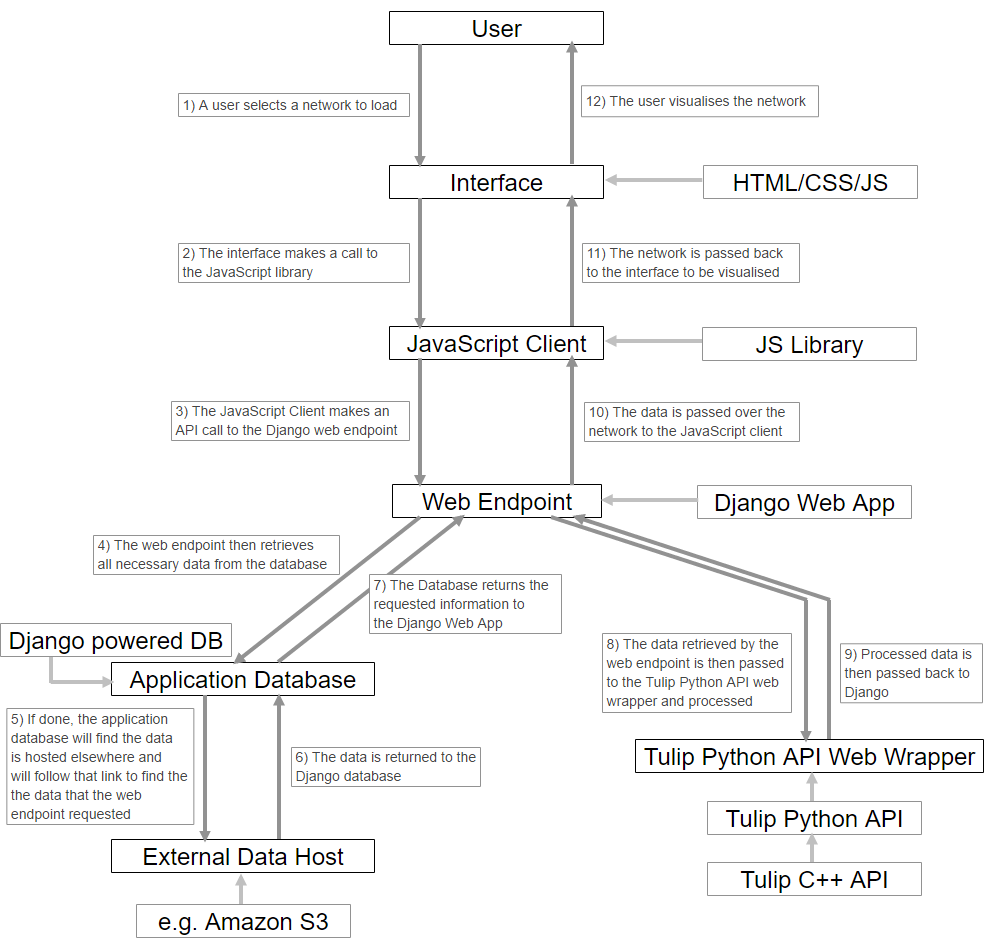
\includegraphics[width=\textwidth]{6/tech_infra_2}
    \caption{The Technical Infrastructure of the whole system, based off the sketch in Appendix \ref{sec:tech_infra_app}}
    \label{fig:techinfra}
    % https://app.moqups.com/ExoBen/rb1XpbcrIp/view/page/ab730d97e?ui=0
\end{figure}

\subsection{Sample Data Flow}

Based on the data flow shown in Figure \ref{fig:techinfra}, the below list was created to show an example of ahow a user could interact with the system, and what the result of those actions would be.

\begin{enumerate}
    \item The user selects a network to open from a list of all networks on the system and clicks on ``Open Network''.
    \item The ID of that network and the request for the network to be loaded is then caught by the JavaScript interface which calls the \texttt{loadGraph} function from the JavaScript library, passing the network ID and a success and error callback.
    \item The JavaScript library makes the appropriate AJAX call to the web endpoint, the Django server.
    \item The Django web application queries the database for the file to load.
    \item If an external data host is set up, then at this point the database would find the location of where the network is stored as opposed to the path the the file locally.
    \item Again, if an external data host is set up, the network would be returned to the application database.
    \item The network is then passed to the web endpoint.
    \item Once the network is loaded into Django, Django then calls a function from the Tulip Python API Web Wrapper and passes it the network. Tulip then loads in the network and then possibly reduces the network using any or all of: node pruning, node bundling based on cliques, or node bundling based on number of edges. Finally, it converts the network into a JsonResponse to be returned.
    \item After the network has been processed and minimised, it is then passed back to the web endpoint again.
    \item From here Django passes either success or failure back to the JavaScript client, with success including the network that is to be visualised, and with failure including a message as to why the network could not be sent back.
    \item The JavaScript library checks if the interface passed in an error callback function. If not then either nothing is returned if the call failed and the network is returned if it is successful. If as error callback function is passed in then if the call failed then JavaScript interface throws an error explaining why the call failed. If everything was successful then Vis.js renders the network.
    \item The user can then examine and explore the visualisation of the network.
\end{enumerate}

\end{document}